% Provenance (never printed): 6e geography and cycle 3 sciences (locating a
% place on the globe: parallels, meridians, latitude, longitude; the Earth's
% rotation and time zones); see sources/book1/PROVENANCE.md.
% Book 1, grade 6, chapter 2.
\chapter{Breedte, lengte en tijdzones}\label{ch:g6:latitude-longitude}

De nacht is gevallen op de \omterm{def:g2:water-on-earth:ocean}{oceaan}. Op het dek van een zeilschip, in het
jaar 1750, heft de navigator zijn instrument naar een heldere ster en meet
hij hoe hoog die boven de \omterm{def:g2:water-on-earth:ocean}{zee} staat. Een paar minuten werk, en hij weet hoe
ver ten noorden van de \omterm{def:g3:continents-and-oceans:equator}{evenaar} het schip is. Maar hoe ver naar het oosten
of het westen? Dat kan hij niet zeggen. Het probleem was zo ernstig dat het
Britse parlement in 1714 een grote prijs had beloofd aan wie een manier
vond om het op \omterm{def:g2:water-on-earth:ocean}{zee} te meten. Vandaag geeft de telefoon in je zak beide
antwoorden in één seconde.
% ledger: rmg:15deg-per-hour, rmg:longitude-act-1714

\begin{omfigure}
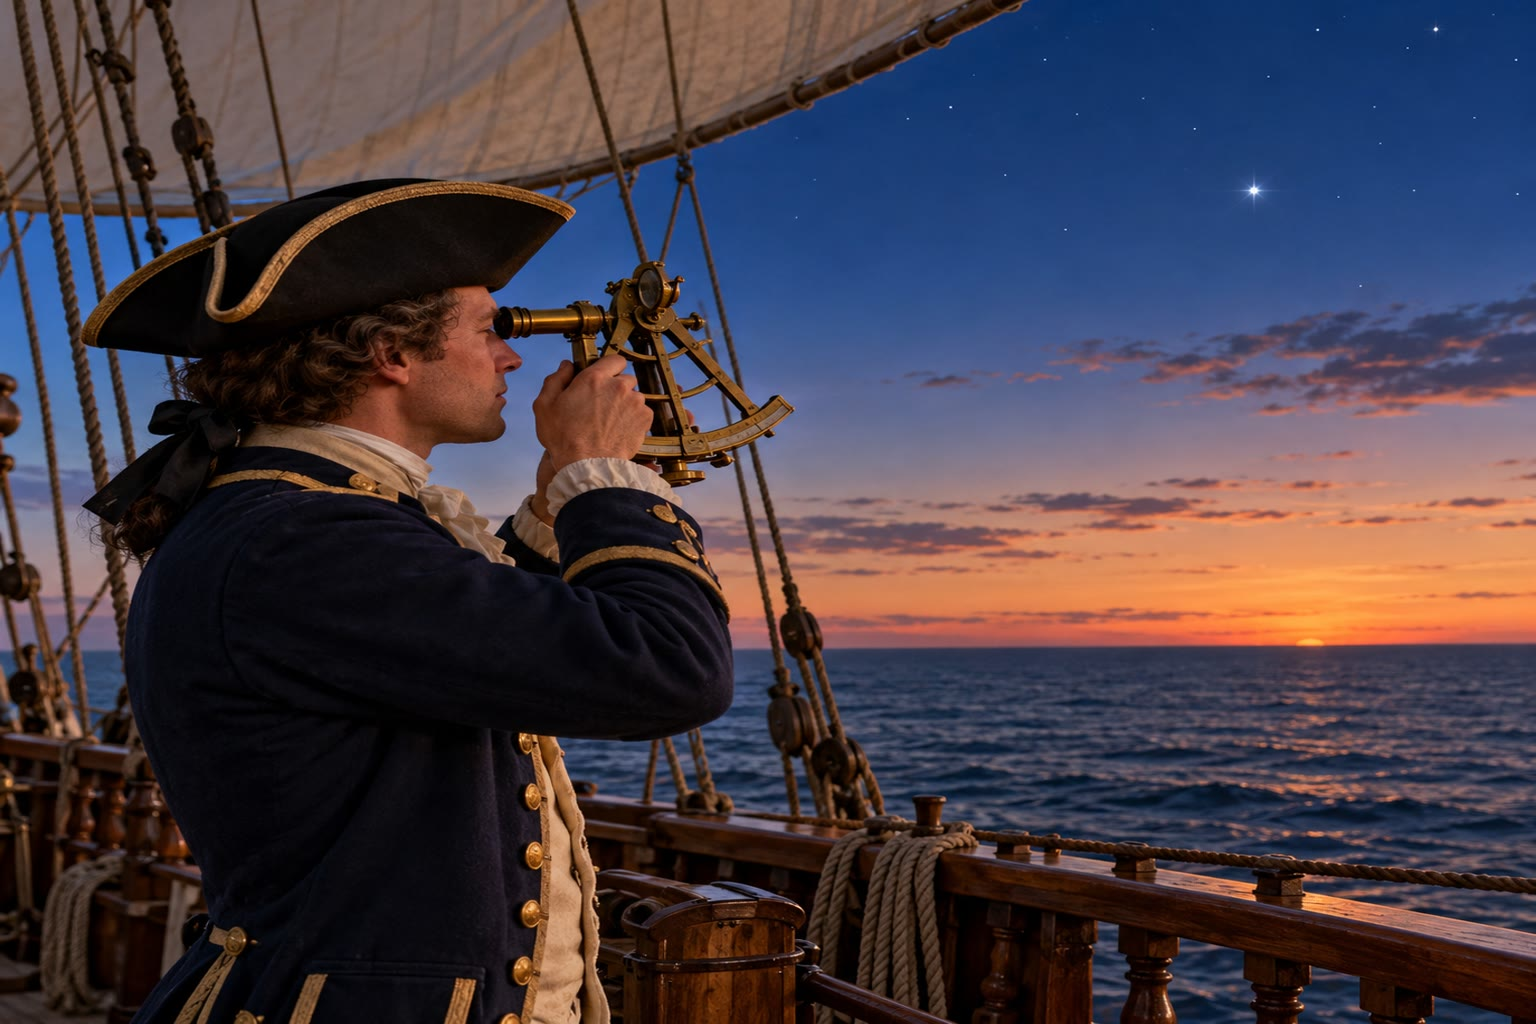
\includegraphics[width=0.62\linewidth]{images/book1/ai/g6-navigator-sextant.jpg}

{\small Een navigator uit de achttiende eeuw meet de hoogte van een ster
boven de zeehorizon. (AI-illustratie.)}
\end{omfigure}

\begin{recall}
Een \omterm{def:g3:continents-and-oceans:globe}{globe} is een klein model van de Aarde. De \omterm{def:g3:continents-and-oceans:equator}{evenaar} is de lijn die rond
het midden van de \omterm{def:g3:continents-and-oceans:globe}{globe} loopt, halverwege tussen de \omterm{def:g3:continents-and-oceans:poles}{Noordpool} en de
\omterm{def:g3:continents-and-oceans:poles}{Zuidpool}; hij snijdt de Aarde in het \omterm{def:g3:continents-and-oceans:equator}{noordelijk halfrond} en het \omterm{def:g3:continents-and-oceans:equator}{zuidelijk
halfrond} (\cref{ch:g3:continents-and-oceans}). De natuurkundeboeken lieten
zien dat de Aarde één keer per dag om zichzelf draait, rond een as door de
twee \omterm{def:g3:continents-and-oceans:poles}{polen}: die draaiing brengt dag en nacht.
\end{recall}

\section{Breedtecirkels en breedtegraad}

Om te zeggen waar een plaats op Aarde ligt, hebben we twee getallen nodig,
zoals de rij en de stoel in een bioscoop. Het eerste zegt hoe ver ten
noorden of ten zuiden van de \omterm{def:g3:continents-and-oceans:equator}{evenaar} de plaats ligt.

Stel je voor dat de Aarde in tweeën wordt gesneden, door beide \omterm{def:g3:continents-and-oceans:poles}{polen}, zoals
een appel die je vanaf het steeltje doorsnijdt. Op het snijvlak (links,
hieronder) is de \omterm{def:g3:continents-and-oceans:equator}{evenaar} de horizontale lijn door het middelpunt. Een
plaats~P aan het oppervlak wordt vanuit het middelpunt gezien onder een
bepaalde hoek boven of onder die lijn: die hoek is haar \omterm{def:g6:latitude-longitude:latitude}{breedtegraad}.

\begin{omfigure}
\begin{minipage}[t]{0.48\linewidth}\centering
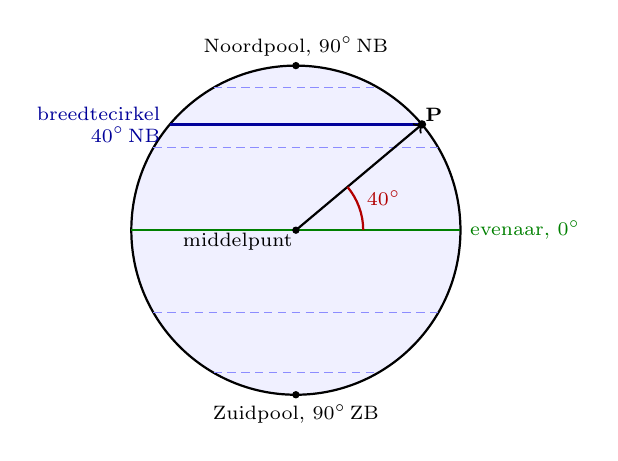
\begin{tikzpicture}[scale=0.95]
  \def\R{2.2}
  \fill[blue!6] (0,0) circle (\R);
  \draw[thick] (0,0) circle (\R);
  % parallels seen edge-on: horizontal chords
  \foreach \a in {-60,-30,30,60}{
    \draw[blue!45, densely dashed] ({-\R*cos(\a)},{\R*sin(\a)}) -- ({\R*cos(\a)},{\R*sin(\a)});}
    \draw[green!50!black, thick] (-\R,0) -- (\R,0);
  \node[font=\scriptsize, green!50!black, anchor=west] at (\R,0) {evenaar, $0^\circ$};
  \draw[blue!60!black, thick] ({-\R*cos(40)},{\R*sin(40)}) -- ({\R*cos(40)},{\R*sin(40)});
  \draw[->, thick] (0,0) -- ({\R*cos(40)},{\R*sin(40)});
  \fill (0,0) circle (1.4pt) node[below left, font=\scriptsize, inner sep=1pt] {middelpunt};
  \fill ({\R*cos(40)},{\R*sin(40)}) circle (1.6pt)
    node[above right, font=\scriptsize\bfseries, inner sep=1pt] {P};
  \draw[red!70!black, thick] (0.9,0) arc (0:40:0.9);
  \node[red!70!black, font=\scriptsize] at (20:1.25) {$40^\circ$};
  \node[font=\scriptsize, blue!60!black, anchor=east, align=right] at ({-\R*cos(40)},{\R*sin(40)}) {breedtecirkel\\$40^\circ$\,NB};
  \fill (0,\R) circle (1.4pt) node[above, font=\scriptsize] {Noordpool, $90^\circ$\,NB};
  \fill (0,-\R) circle (1.4pt) node[below, font=\scriptsize] {Zuidpool, $90^\circ$\,ZB};
\end{tikzpicture}

{\small \omterm{def:g6:latitude-longitude:latitude}{Breedtegraad}: de hoek in het middelpunt van de Aarde tussen de
\omterm{def:g3:continents-and-oceans:equator}{evenaar} en de plaats.}
\end{minipage}\hfill
\begin{minipage}[t]{0.48\linewidth}\centering
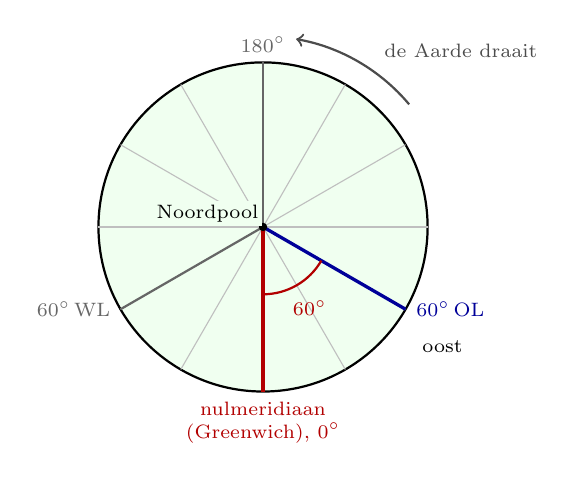
\begin{tikzpicture}[scale=0.95]
  \def\R{2.2}
  \fill[green!6] (0,0) circle (\R);
  \draw[thick] (0,0) circle (\R);
  \foreach \a in {0,30,...,330}{\draw[black!25] (0,0) -- (\a:\R);}
    \draw[red!70!black, very thick] (0,0) -- (270:\R)
    node[below, font=\scriptsize, align=center] {nulmeridiaan\\(Greenwich), $0^\circ$};
  \draw[blue!60!black, very thick] (0,0) -- (330:\R)
    node[right, font=\scriptsize] {$60^\circ$\,OL};
  \draw[black!60, thick] (0,0) -- (210:\R) node[left, font=\scriptsize] {$60^\circ$\,WL};
  \draw[black!60, thick] (0,0) -- (90:\R) node[above, font=\scriptsize] {$180^\circ$};
  \draw[red!70!black, thick] (270:0.9) arc (270:330:0.9);
  \node[red!70!black, font=\scriptsize] at (300:1.25) {$60^\circ$};
    \fill (0,0) circle (1.6pt) node[above left, font=\scriptsize, inner sep=1.5pt, fill=green!6] {Noordpool};
  \draw[->, thick, black!70] (40:2.55) arc (40:80:2.55);
  \node[font=\scriptsize, black!70, anchor=south west] at (55:2.6) {de Aarde draait};
  \node[font=\scriptsize, anchor=west] at (2.0,-1.6) {oost $\circlearrowleft$};
\end{tikzpicture}

{\small \omterm{def:g6:latitude-longitude:longitude}{Lengtegraad}: de Aarde gezien van boven de \omterm{def:g3:continents-and-oceans:poles}{Noordpool}. De hoek wordt
gemeten vanaf de \omterm{def:g6:latitude-longitude:longitude}{nulmeridiaan}, naar het oosten of naar het westen.}
\end{minipage}
% ledger: rmg:latitude-def, rmg:longitude-def
\end{omfigure}

\begin{definition}[Breedtecirkel en breedtegraad]\label{def:g6:latitude-longitude:latitude}
Een \emph{breedtecirkel}\index{breedtecirkel} is een cirkel rond de \omterm{def:g3:continents-and-oceans:globe}{globe},
evenwijdig aan de \omterm{def:g3:continents-and-oceans:equator}{evenaar}; alle plaatsen op dezelfde breedtecirkel liggen
even ver van de \omterm{def:g3:continents-and-oceans:equator}{evenaar}. De \emph{breedtegraad}\index{breedtegraad} van een
plaats is de hoek, gemeten in het middelpunt van de Aarde, tussen de
\omterm{def:g3:continents-and-oceans:equator}{evenaar} en die plaats. Hij loopt van $0^\circ$ op de \omterm{def:g3:continents-and-oceans:equator}{evenaar} tot $90^\circ$
op de \omterm{def:g3:continents-and-oceans:poles}{polen}, en we zeggen of de plaats ten noorden (noorderbreedte, NB) of
ten zuiden (zuiderbreedte, ZB) van de \omterm{def:g3:continents-and-oceans:equator}{evenaar} ligt.
% ledger: rmg:latitude-def
\end{definition}

De \omterm{def:g3:continents-and-oceans:equator}{evenaar} is zelf een \omterm{def:g6:latitude-longitude:latitude}{breedtecirkel}, de langste, met \omterm{def:g6:latitude-longitude:latitude}{breedtegraad}
$0^\circ$. De \omterm{def:g6:latitude-longitude:latitude}{breedtecirkels} worden korter naar de \omterm{def:g3:continents-and-oceans:poles}{polen} toe, en elke \omterm{def:g3:continents-and-oceans:poles}{pool}
is één punt, op $90^\circ$\,NB of $90^\circ$\,ZB. Langs een lijn van een
\omterm{def:g3:continents-and-oceans:poles}{pool} naar de \omterm{def:g3:continents-and-oceans:equator}{evenaar} is elke \omterm{def:g6:latitude-longitude:latitude}{breedtegraad} ongeveer \qty{111}{km}.
% ledger: rmg:latitude-def

De \omterm{def:g6:latitude-longitude:latitude}{breedtegraad} is het makkelijke getal: je vindt hem aan de hemel. Overdag
maten zeelieden de hoogte van de Zon om twaalf uur 's middags; 's nachts,
op het \omterm{def:g3:continents-and-oceans:equator}{noordelijk halfrond}, maten ze de hoogte van de Poolster. Dat is wat
de navigator op het plaatje aan het begin doet.
% ledger: rmg:15deg-per-hour

De Poolster staat bijna precies op het verlengde van de aardas, voorbij de
\omterm{def:g3:continents-and-oceans:poles}{Noordpool}, en zo ver weg dat haar licht elke plaats op Aarde langs
evenwijdige lijnen bereikt. Op de \omterm{def:g3:continents-and-oceans:poles}{Noordpool} staat ze recht boven je hoofd,
op $90^\circ$ boven de horizon; op de \omterm{def:g3:continents-and-oceans:equator}{evenaar} staat ze op de noordelijke
horizon, op $0^\circ$. Daartussen is de regel eenvoudig: \emph{de hoogte
van de Poolster boven de noordelijke horizon, gemeten als hoek, is gelijk
aan de \omterm{def:g6:latitude-longitude:latitude}{breedtegraad}}. De figuur hieronder laat zien waarom de twee hoeken
gelijk zijn.
% ledger: nsta:polaris-latitude

\begin{omfigure}
\begin{tikzpicture}[scale=1.1, font=\scriptsize]
  \def\R{1.7}
  \coordinate (O) at (0,0);
  \coordinate (P) at ({\R*cos(40)},{\R*sin(40)});
  \fill[blue!8] (O) circle (\R);
  \draw[black!70] (O) circle (\R);
  % equator and axis
  \draw[black!50] (-\R,0) -- (\R,0);
  \node[black!60, anchor=north east] at (-0.15,0) {evenaar};
  \draw[black!70, -{Stealth[length=2mm]}] (0,-\R-0.3) -- (0,\R+1.7);
  \node[anchor=east, align=right] at (-0.1,\R+1.45) {naar de Poolster\\(heel ver weg)};
  \node[anchor=south east] at (0,\R) {N};
  % radius to P and latitude angle at the centre
  \draw[black!80] (O) -- (P);
  \draw[red!70!black, thick] (0.55,0) arc (0:40:0.55);
  \node[red!70!black] at (20:0.8) {$40^\circ$};
  % horizon at P (tangent) and the ray to the Pole Star (parallel to the axis)
  \draw[black!70, thick] ($(P)+({-sin(40)*1.5},{cos(40)*1.5})$) -- ($(P)+({sin(40)*1.6},{-cos(40)*1.6})$);
  \node[anchor=south, rotate=-50, inner sep=2pt] at ($(P)+({sin(40)*1.15},{-cos(40)*1.15})$) {horizon};
  \draw[orange!80!black, thick, -{Stealth[length=2mm]}] (P) -- ++(0,1.45);
  \draw[red!70!black, thick] ($(P)+(0,0.7)$) arc (90:130:0.7);
  \node[red!70!black] at ($(P)+(110:0.98)$) {$40^\circ$};
  \fill (P) circle (1.4pt);
  \node[anchor=west] at ($(P)+(0.3,0.05)$) {waarnemer op $40^\circ$\,NB};
\end{tikzpicture}

{\small Waarom de hoogte van de Poolster gelijk is aan de \omterm{def:g6:latitude-longitude:latitude}{breedtegraad} (een
schets, niet op schaal). Het licht van de Poolster komt evenwijdig aan de
aardas aan (oranje). De horizon van de waarnemer staat loodrecht op de
straal door de waarnemer; de as staat loodrecht op de \omterm{def:g3:continents-and-oceans:equator}{evenaar}. Dus is de
hoek tussen de horizon en de Poolster gelijk aan de \omterm{def:g6:latitude-longitude:latitude}{breedtegraad}, de hoek
in het middelpunt tussen de \omterm{def:g3:continents-and-oceans:equator}{evenaar} en de waarnemer.}
% ledger: nsta:polaris-latitude
\end{omfigure}

\begin{example}[Een navigator in de nacht]\label{ex:g6:latitude-longitude:pole-star}
Een navigator meet de Poolster op $41^\circ$ boven de noordelijke horizon.
Het schip ligt op $41^\circ$\,NB, ongeveer $41 \times 111
\approx \num{4550}$~km ten noorden van de \omterm{def:g3:continents-and-oceans:equator}{evenaar}. Als ze naar het noorden
vaart, staat de ster elke nacht een beetje hoger; als ze naar het zuiden
vaart, naar de \omterm{def:g3:continents-and-oceans:equator}{evenaar}, zakt hij naar de horizon. Ten zuiden van de \omterm{def:g3:continents-and-oceans:equator}{evenaar}
is de Poolster helemaal niet te zien, want ze blijft onder de horizon: daar
geeft de middagzon de \omterm{def:g6:latitude-longitude:latitude}{breedtegraad}.
\end{example}
% ledger: nsta:polaris-latitude, rmg:latitude-def, rmg:15deg-per-hour

\section{Meridianen en lengtegraad}

Het tweede getal zegt hoe ver naar het oosten of het westen een plaats ligt.
Hier is er geen natuurlijke beginlijn zoals de \omterm{def:g3:continents-and-oceans:equator}{evenaar}: er moet er een
worden gekozen.

\begin{definition}[Meridiaan, lengtegraad en nulmeridiaan]\label{def:g6:latitude-longitude:longitude}
Een \emph{meridiaan}\index{meridiaan} is een halve cirkel op de \omterm{def:g3:continents-and-oceans:globe}{globe} van de
\omterm{def:g3:continents-and-oceans:poles}{Noordpool} naar de \omterm{def:g3:continents-and-oceans:poles}{Zuidpool}. De \emph{nulmeridiaan}\index{nulmeridiaan} is
de meridiaan die als beginlijn is gekozen: die door de oude Koninklijke
Sterrenwacht van Greenwich, in Londen. De
\emph{lengtegraad}\index{lengtegraad} van een plaats is de hoek tussen de
nulmeridiaan en de meridiaan van die plaats, gezien vanaf de aardas. Hij
loopt van $0^\circ$ op de nulmeridiaan tot $180^\circ$, en we zeggen of de
plaats ten oosten (oosterlengte, OL) of ten westen (westerlengte, WL) van
de nulmeridiaan ligt.
% ledger: rmg:longitude-def
\end{definition}

Alle \omterm{def:g6:latitude-longitude:longitude}{meridianen} komen samen op de \omterm{def:g3:continents-and-oceans:poles}{polen}, en ze zijn allemaal even lang. Aan
de andere kant van de Aarde, tegenover Greenwich, zijn de \omterm{def:g6:latitude-longitude:longitude}{meridiaan}
$180^\circ$\,OL en de \omterm{def:g6:latitude-longitude:longitude}{meridiaan} $180^\circ$\,WL dezelfde lijn.

\begin{omfigure}
\begin{minipage}[c]{0.46\linewidth}\centering
\begin{tikzpicture}
  \begin{axis}[axis equal image, hide axis, width=\linewidth,
      xmin=-1.05, xmax=1.05, ymin=-1.05, ymax=1.12, clip=false]
    \fill[omSea] (axis cs:0,0) circle (1);
    \addplot[fill=omLithAlluv, draw=black!45, line width=0.2pt] table {figdata/out/grade-6-graticule-land.dat};
    \addplot[blue!50!black, line width=0.35pt] table {figdata/out/grade-6-graticule-parallels.dat};
    \addplot[black!55, line width=0.35pt] table {figdata/out/grade-6-graticule-meridians.dat};
        \addplot[green!50!black, line width=1.1pt] table {figdata/out/grade-6-graticule-equator.dat};
    \addplot[red!70!black, line width=1.1pt] table {figdata/out/grade-6-graticule-prime.dat};
    \draw[black!70] (axis cs:0,0) circle (1);
    \fill (axis cs:0,0.9063) circle (1.3pt);
        \node[font=\scriptsize, above left, inner sep=1.5pt] at (axis cs:0,0.9063) {N};
  \end{axis}
\end{tikzpicture}
\end{minipage}\hfill
\begin{minipage}[c]{0.5\linewidth}
{\small Een \omterm{def:g3:continents-and-oceans:globe}{globe} met zijn \omterm{def:g6:latitude-longitude:latitude}{breedtecirkels} (blauw) en \omterm{def:g6:latitude-longitude:longitude}{meridianen} (grijs), om
de $30^\circ$. De \omterm{def:g3:continents-and-oceans:equator}{evenaar} is dik groen getekend, de \omterm{def:g6:latitude-longitude:longitude}{nulmeridiaan} rood; ze
kruisen elkaar in de \omterm{def:g2:water-on-earth:ocean}{oceaan} ten zuiden van Ghana, op breedte $0^\circ$,
lengte $0^\circ$. Elke \omterm{def:g6:latitude-longitude:longitude}{meridiaan} loopt van \omterm{def:g3:continents-and-oceans:poles}{pool} tot \omterm{def:g3:continents-and-oceans:poles}{pool}; elke \omterm{def:g6:latitude-longitude:latitude}{breedtecirkel}
is een cirkel rond de as. (Land: Natural Earth.)}
% ledger: data:ne-land (figdata/grade-6/graticule.py)
\end{minipage}
\end{omfigure}

\begin{history}[De keuze van de nulmeridiaan]
Lange tijd tekende elk land zijn \omterm{def:g2:drawing-to-map:map}{kaarten} met zijn eigen beginmeridiaan:
Londen, Parijs en andere plaatsen werden allemaal gebruikt. In oktober 1884
kwamen afgevaardigden van veel landen in Washington bijeen om één
\omterm{def:g6:latitude-longitude:longitude}{meridiaan} voor de hele wereld te kiezen. Op 13~oktober stemden ze om de
\omterm{def:g6:latitude-longitude:longitude}{meridiaan} door de sterrenwacht van Greenwich voor te stellen: 21 landen
stemden voor, één tegen, en twee stemden niet.
% ledger: rmg:longitude-def, meridian:1884-vote
\end{history}

\section{Een plaats vinden met haar twee hoeken}

Met haar \omterm{def:g6:latitude-longitude:latitude}{breedtegraad} en haar \omterm{def:g6:latitude-longitude:longitude}{lengtegraad} kun je elke plaats op Aarde
terugvinden, op een \omterm{def:g2:drawing-to-map:map}{kaart} of op een \omterm{def:g3:continents-and-oceans:globe}{globe}. We schrijven de breedte eerst:
Caïro bijvoorbeeld ligt op ongeveer $30^\circ$\,NB, $31^\circ$\,OL.
% ledger: data:b1-ne-places (figdata/grade-6/cities.py)

\begin{omfigure}
\begin{tikzpicture}
  \begin{axis}[ommap, width=\linewidth,
      xtick={-180,-150,...,180}, ytick={-90,-60,...,90},
      xticklabels={$180^\circ$,$150^\circ$WL,$120^\circ$WL,$90^\circ$WL,$60^\circ$WL,$30^\circ$WL,$0^\circ$,
                   $30^\circ$OL,$60^\circ$OL,$90^\circ$OL,$120^\circ$OL,$150^\circ$OL,$180^\circ$},
      yticklabels={$90^\circ$ZB,$60^\circ$ZB,$30^\circ$ZB,$0^\circ$,$30^\circ$NB,$60^\circ$NB,$90^\circ$NB},
      tick label style={font=\tiny}, grid style={black!35, line width=0.3pt}]
    \addplot[fill=omLithAlluv, draw=black!45, line width=0.2pt] table {figdata/out/shared-geo-land.dat};
        \draw[green!50!black, line width=0.9pt] (axis cs:-180,0) -- (axis cs:180,0);
    \draw[red!70!black, line width=0.9pt] (axis cs:0,-90) -- (axis cs:0,90);
    \addplot[only marks, mark=*, mark size=1.2pt, black,
        point meta=explicit symbolic,
        visualization depends on={value \thisrow{anchor}\as\anc},
        nodes near coords, nodes near coords style={font=\tiny, inner sep=1.2pt,
          anchor=\anc, fill=white, fill opacity=0.75, text opacity=1}]
      table[x=lon, y=lat, meta=name, row sep=\\] {lon lat name anchor\\ -21.936 64.144 Reykjavík south\\ -0.119 51.502 Londen south\\ -73.996 40.722 New~York west\\ -118.232 34.049 Los~Angeles east\\ -78.502 -0.213 Quito east\\ -43.212 -22.907 Rio~de~Janeiro west\\ 18.433 -33.918 Kaapstad north\\ 36.815 -1.281 Nairobi west\\ 31.248 30.052 Caïro south\\ 72.876 19.068 Mumbai north\\ 139.75 35.687 Tokio west\\ 151.213 -33.871 Sydney south\\ 174.763 -36.848 Auckland {north east}\\ };
  \end{axis}
\end{tikzpicture}

{\small Dertien steden op een \omterm{def:g3:continents-and-oceans:world-map}{wereldkaart} met een raster om de $30^\circ$.
De \omterm{def:g3:continents-and-oceans:equator}{evenaar} is groen getekend, de \omterm{def:g6:latitude-longitude:longitude}{nulmeridiaan} rood. (Kustlijnen en steden:
Natural Earth.)}
% ledger: data:ne-land, data:b1-ne-places (figdata/grade-6/cities.py, part map)
\end{omfigure}

\begin{method}[Een plaats vinden met haar coördinaten]\label{met:g6:latitude-longitude:locating}
\begin{enumerate}
  \item \omterm{def:g6:latitude-longitude:latitude}{Breedtegraad}: begin bij de \omterm{def:g3:continents-and-oceans:equator}{evenaar} en ga naar het noorden (NB) of
        het zuiden (ZB), terwijl je de \omterm{def:g6:latitude-longitude:latitude}{breedtecirkels} telt, tot het juiste
        aantal graden.
  \item \omterm{def:g6:latitude-longitude:longitude}{Lengtegraad}: begin bij de \omterm{def:g6:latitude-longitude:longitude}{nulmeridiaan} en ga naar het oosten (OL)
        of het westen (WL), terwijl je de \omterm{def:g6:latitude-longitude:longitude}{meridianen} telt, tot het juiste
        aantal graden.
  \item De plaats ligt waar de \omterm{def:g6:latitude-longitude:latitude}{breedtecirkel} en de \omterm{def:g6:latitude-longitude:longitude}{meridiaan} elkaar
        kruisen. Tussen twee lijnen van het raster schat je: halverwege
        tussen $30^\circ$ en $60^\circ$ is $45^\circ$.
\end{enumerate}
\end{method}

\begin{example}[De coördinaten van Sydney aflezen]\label{ex:g6:latitude-longitude:sydney}
Op de \omterm{def:g2:drawing-to-map:map}{kaart} ligt Sydney onder de \omterm{def:g3:continents-and-oceans:equator}{evenaar}: het ligt op het \omterm{def:g3:continents-and-oceans:equator}{zuidelijk
halfrond}, iets boven de \omterm{def:g6:latitude-longitude:latitude}{breedtecirkel} $30^\circ$\,ZB, dichter bij $30^\circ$
dan bij $60^\circ$; de \omterm{def:g6:latitude-longitude:latitude}{breedtegraad} is ongeveer $34^\circ$\,ZB. Het ligt
rechts van de \omterm{def:g6:latitude-longitude:longitude}{nulmeridiaan}, iets voorbij de \omterm{def:g6:latitude-longitude:longitude}{meridiaan} $150^\circ$\,OL; de
\omterm{def:g6:latitude-longitude:longitude}{lengtegraad} is ongeveer $151^\circ$\,OL. We schrijven: Sydney,
$34^\circ$\,ZB, $151^\circ$\,OL.
% ledger: data:b1-ne-places (cities.py: 33.87 S, 151.21 E)
\end{example}

\section{De draaiende Aarde en de tijdzones}

De Aarde draait één keer per dag om zichzelf, van west naar oost. Terwijl
ze draait, lijkt de Zon van oost naar west langs de hemel te trekken. Als
de Zon op haar hoogst aan de hemel staat, is het twaalf uur 's middags.
Maar het is niet overal op hetzelfde moment middag: als het in Londen
twaalf uur 's middags is, is het in Caïro, verder naar het oosten, al na
twaalven, en in New York, verder naar het westen, nog ochtend.

Hoeveel draait de Aarde in één uur? Een hele omwenteling is $360^\circ$, en
die duurt 24~uur:
\[
360^\circ \div 24 = 15^\circ \text{ per uur.}
\]
Twee plaatsen die $15^\circ$ lengte uit elkaar liggen, hebben hun middag
dus een uur na elkaar: de plaats die oostelijker ligt, heeft hem het eerst.
Eén graad duurt 4~minuten.
% ledger: planet:Earth.day, rmg:15deg-per-hour

\begin{definition}[Tijdzone]\label{def:g6:latitude-longitude:time-zone}
Een \emph{tijdzone}\index{tijdzone} is een strook van de Aarde, van \omterm{def:g3:continents-and-oceans:poles}{pool}
tot \omterm{def:g3:continents-and-oceans:poles}{pool}, waar alle klokken dezelfde tijd aanwijzen. In het ideale geval is
elke zone $15^\circ$ lengte breed, zodat er 24 zones zijn, één voor elk
uur; als je één zone naar het oosten gaat, wijzen de klokken een uur later
aan.
\end{definition}

In de ideale zones is de zone van een plaats haar \omterm{def:g6:latitude-longitude:longitude}{lengtegraad} gedeeld door
$15$, afgerond op een heel getal: ten oosten van Greenwich tellen we dat
aantal uren op bij de tijd in Greenwich, ten westen ervan trekken we ze
eraf. Tokio, op $140^\circ$\,OL: $140 \div 15 \approx 9.3$, dus de zone is
$+9$: als het in Greenwich twaalf uur 's middags is, is het in Tokio
21~uur. Echte \omterm{def:g6:latitude-longitude:time-zone}{tijdzones} zijn geen rechte stroken: ze volgen de grenzen van
landen en regio's, zodat een heel land, of een hele regio, dezelfde tijd
houdt.
% ledger: data:b1-ne-places, rmg:15deg-per-hour

\begin{omfigure}
\begin{tikzpicture}
  \begin{axis}[ommap, width=\linewidth, clip=false,
      xtick={-180,-90,0,90,180}, ytick={-60,0,60},
      xticklabels={$180^\circ$,$90^\circ$WL,$0^\circ$,$90^\circ$OL,$180^\circ$},
      yticklabels={$60^\circ$ZB,$0^\circ$,$60^\circ$NB},
      tick label style={font=\tiny}, grid=none]
    \addplot[fill=black!8, draw=none] table {figdata/out/grade-6-time_zones-odd.dat};
    \addplot[fill=omLithAlluv, fill opacity=0.85, draw=black!45, line width=0.2pt] table {figdata/out/shared-geo-land.dat};
    \addplot[only marks, mark=none, point meta=explicit symbolic,
        nodes near coords, nodes near coords style={font=\tiny, anchor=south, inner sep=1pt}]
            table[x=lon, y=y, meta=label] {figdata/out/grade-6-time_zones-labels.dat};
    \draw[red!75!black, line width=1.6pt] (axis cs:180,-90) -- (axis cs:180,90);
    \draw[red!75!black, line width=1.6pt] (axis cs:-180,-90) -- (axis cs:-180,90);
        \draw[black, line width=0.8pt] (axis cs:0,-90) -- (axis cs:0,90);
    \node[font=\scriptsize, red!75!black, rotate=90, anchor=south] at (axis cs:180,0) {datumgrens};
    \node[font=\scriptsize, red!75!black, rotate=90, anchor=north] at (axis cs:-180,0) {datumgrens};
  \end{axis}
\end{tikzpicture}

{\small De 24 ideale \omterm{def:g6:latitude-longitude:time-zone}{tijdzones}, elk $15^\circ$ breed, met het aantal uren
dat je moet optellen bij de tijd in Greenwich (de zwarte lijn in het
midden). De \omterm{def:g6:latitude-longitude:date-line}{datumgrens} loopt langs de \omterm{def:g6:latitude-longitude:longitude}{meridiaan} van $180^\circ$, die deze
\omterm{def:g2:drawing-to-map:map}{kaart} in tweeën snijdt: hij is zowel de linker- als de rechterrand. Rol de
\omterm{def:g2:drawing-to-map:map}{kaart} op tot een koker, en de twee rode lijnen worden één. De zone aan
weerszijden van de \omterm{def:g6:latitude-longitude:date-line}{datumgrens} is een halve zone breed.}
% ledger: rmg:15deg-per-hour, planet:Earth.day (figdata/grade-6/time_zones.py)
\end{omfigure}

\paragraph{De datumgrens.} Reis vanuit Greenwich naar het oosten en tel
per zone een uur op: op $180^\circ$ loop je 12~uur voor. Reis naar het
westen en trek per zone een uur af: op $180^\circ$ loop je 12~uur achter.
De twee reizigers ontmoeten elkaar op dezelfde \omterm{def:g6:latitude-longitude:longitude}{meridiaan}, met klokken die
hetzelfde uur aanwijzen, maar een hele dag uit elkaar! Een van hen moet de
datum veranderen.

\begin{definition}[Internationale datumgrens]\label{def:g6:latitude-longitude:date-line}
De \emph{internationale datumgrens}\index{internationale datumgrens} is de
lijn, midden in de Stille \omterm{def:g2:water-on-earth:ocean}{Oceaan}, waar de datum verandert. Hij volgt de
\omterm{def:g6:latitude-longitude:longitude}{meridiaan} van $180^\circ$, met een paar bochten om geen land in tweeën te
snijden. Als je hem naar het westen oversteekt, ga je naar de volgende
dag; als je hem naar het oosten oversteekt, ga je terug naar de dag
ervoor.
\end{definition}

\begin{history}[Het zeehorloge van Harrison]
\begin{minipage}[c]{0.7\linewidth}
Om zijn \omterm{def:g6:latitude-longitude:longitude}{lengtegraad} te vinden, vergelijkt een navigator twee tijden: de
plaatselijke tijd op het schip, afgelezen aan de Zon, en op hetzelfde
moment de tijd in een thuishaven. Elk uur verschil betekent $15^\circ$
lengte. De moeilijkheid was om de thuistijd over de \omterm{def:g2:water-on-earth:ocean}{oceaan} mee te nemen:
zelfs de beste horloges van die tijd waren niet nauwkeurig genoeg. De
Engelse klokkenmaker John Harrison werkte tientallen jaren aan het
probleem, met als doel een klok die per dag niet meer dan 3~seconden voor
of achter zou gaan. Zijn vierde zeeklok, H4 genoemd, lijkt op een groot
zakhorloge en tikt vijf keer per seconde. In 1761 nam zijn zoon William
hem mee op een reis naar Jamaica om hem te testen.
% ledger: rmg:15deg-per-hour, rmg:longitude-act-1714, rmg:h4-jamaica-1761
\end{minipage}\hfill
\begin{minipage}[c]{0.26\linewidth}\centering
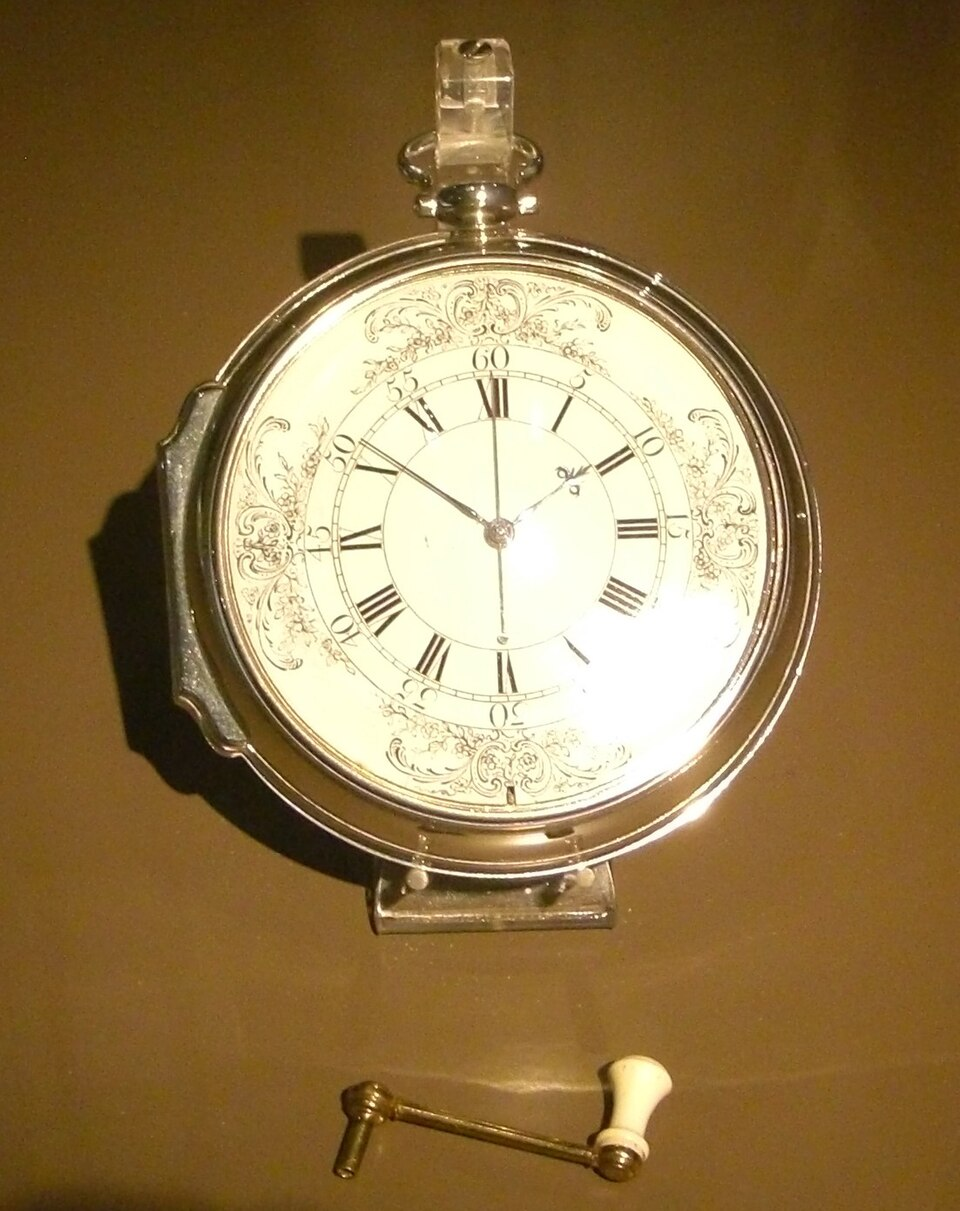
\includegraphics[width=\linewidth]{images/book1/g6-harrison-h4.jpg}\\[2pt]
{\footnotesize De H4 van Harrison, National Maritime Museum, Greenwich.
(Foto: Colonel Warden, CC BY-SA 3.0, via Wikimedia Commons.)}
% ledger: commons:harrison-h4
\end{minipage}
\end{history}

\section{Oefeningen}

\begin{exercise}[$\star$]\label{exo:g6:latitude-longitude:1}
Neem over en vul aan: ``De \omterm{def:g6:latitude-longitude:latitude}{breedtegraad} wordt gemeten vanaf de \ldots{} en
loopt van $0^\circ$ tot \ldots; de \omterm{def:g6:latitude-longitude:longitude}{lengtegraad} wordt gemeten vanaf de
\ldots{} en loopt van $0^\circ$ tot \ldots''
\end{exercise}

\begin{exercise}[$\star$]\label{exo:g6:latitude-longitude:2}
Wat is de \omterm{def:g6:latitude-longitude:latitude}{breedtegraad} van de \omterm{def:g3:continents-and-oceans:poles}{Noordpool}? En van de \omterm{def:g3:continents-and-oceans:poles}{Zuidpool}? En van een
stad op de \omterm{def:g3:continents-and-oceans:equator}{evenaar}?
\end{exercise}

\begin{exercise}[$\star$]\label{exo:g6:latitude-longitude:3}
Zeg met de \omterm{def:g2:drawing-to-map:map}{kaart} van de dertien steden op welk \omterm{def:g3:continents-and-oceans:equator}{halfrond}, noordelijk of
zuidelijk, en aan welke kant van de \omterm{def:g6:latitude-longitude:longitude}{nulmeridiaan}, oost of west, elk van
deze steden ligt: Sydney, New York, Caïro, Rio de Janeiro.
\end{exercise}

\begin{exercise}[$\star$]\label{exo:g6:latitude-longitude:4}
Waar of niet waar? Verbeter de zinnen die niet waar zijn.
(a) Alle \omterm{def:g6:latitude-longitude:longitude}{meridianen} komen samen op de \omterm{def:g3:continents-and-oceans:poles}{polen}.
(b) Alle \omterm{def:g6:latitude-longitude:latitude}{breedtecirkels} zijn even lang.
(c) De \omterm{def:g3:continents-and-oceans:equator}{evenaar} is een \omterm{def:g6:latitude-longitude:latitude}{breedtecirkel}.
(d) De \omterm{def:g6:latitude-longitude:longitude}{nulmeridiaan} loopt door Parijs.
\end{exercise}

\begin{exercise}[$\star\star$]\label{exo:g6:latitude-longitude:5}
Welke stad ligt volgens de \omterm{def:g2:drawing-to-map:map}{kaart} van de dertien steden op ongeveer
$30^\circ$\,NB, $31^\circ$\,OL? Welke op ongeveer $41^\circ$\,NB,
$74^\circ$\,WL? Geef de geschatte coördinaten van Tokio.
% ledger: data:b1-ne-places (cities.py main table)
\end{exercise}

\begin{exercise}[$\star\star$]\label{exo:g6:latitude-longitude:6}
Stad~A ligt op \omterm{def:g6:latitude-longitude:longitude}{lengtegraad} $0^\circ$ en stad~B op $45^\circ$\,OL. Hoeveel
uur liggen hun middagen uit elkaar? In welke stad is het het eerst middag?
\end{exercise}

\begin{exercise}[$\star\star$]\label{exo:g6:latitude-longitude:7}
Mumbai ligt op ongeveer $73^\circ$\,OL. Bereken de ideale \omterm{def:g6:latitude-longitude:time-zone}{tijdzone}. Hoe laat
is het in Mumbai, in de ideale zones, als het in Greenwich twaalf uur
's middags is?
% ledger: data:b1-ne-places (cities.py: 72.88 E, zone +5)
\end{exercise}

\begin{exercise}[$\star\star$]\label{exo:g6:latitude-longitude:8}
Elke \omterm{def:g6:latitude-longitude:latitude}{breedtegraad} is ongeveer \qty{111}{km}. Hoe ver van de \omterm{def:g3:continents-and-oceans:equator}{evenaar} ligt
een stad op $30^\circ$\,NB, gemeten langs haar \omterm{def:g6:latitude-longitude:longitude}{meridiaan}? Hoe ver ligt de
\omterm{def:g3:continents-and-oceans:poles}{Noordpool} van de \omterm{def:g3:continents-and-oceans:equator}{evenaar}?
% ledger: rmg:latitude-def
\end{exercise}

\begin{exercise}[$\star\star$]\label{exo:g6:latitude-longitude:9}
New York ligt in de zone $-5$ en Tokio in de zone $+9$. Hoeveel uur
verschillen hun klokken? Als het in New York maandag 8~uur 's ochtends is,
hoe laat en welke dag is het dan in Tokio?
% ledger: data:b1-ne-places (cities.py: zones -5 and +9)
\end{exercise}

\begin{exercise}[$\star\star$]\label{exo:g6:latitude-longitude:10}
Lena zegt: ``De Zon komt op in het oosten, dus de steden in het oosten zien
de Zon eerder opkomen dan de steden in het westen.'' Heeft ze gelijk? Leg
uit met de draaiing van de Aarde.
\end{exercise}

\begin{exercise}[$\star\star\star$]\label{exo:g6:latitude-longitude:11}
Een scheepsklok loopt 3~seconden per dag voor (ze loopt te snel).
(a) Hoeveel seconden loopt ze voor na een reis van 42~dagen? (b) De Aarde
draait één graad in 4~minuten, dat is 240~seconden. Welke fout, in graden
lengte, veroorzaakt de fout van de klok? (c) Op de \omterm{def:g3:continents-and-oceans:equator}{evenaar} is één
\omterm{def:g6:latitude-longitude:longitude}{lengtegraad} ongeveer \qty{111}{km}. Hoeveel kilometer zit de navigator er
op de \omterm{def:g3:continents-and-oceans:equator}{evenaar} ongeveer naast?
% ledger: rmg:longitude-act-1714, rmg:15deg-per-hour, rmg:latitude-def
\end{exercise}

\begin{exercise}[$\star\star\star$]\label{exo:g6:latitude-longitude:12}
Een vliegtuig vertrekt op maandag om 18~uur uit Tokio (zone $+9$) en
vliegt naar het oosten over de Stille \omterm{def:g2:water-on-earth:ocean}{Oceaan} naar Los Angeles (zone $-8$).
De vlucht duurt 10~uur. (a) Hoe laat is het in Greenwich als het vliegtuig
vertrekt? (b) Hoe laat is het in Greenwich als het landt? (c) Wat is de
plaatselijke tijd en de dag in Los Angeles als het landt? Waarom zeggen
reizigers dat je op deze vlucht ``landt voordat je vertrokken bent''?
\end{exercise}

\section{Probleem: Een videogesprek rond de wereld}

\begin{problem}[{Weekendprobleem --- vijf vrienden, vier tijdzones en één
datumgrens: hoe laat is het in Auckland als het gesprek begint?}]
\label{pb:g6:latitude-longitude:1}
% ledger: data:b1-ne-places, rmg:15deg-per-hour, planet:Earth.day (cities.py, time_zones.py; test_cities_zones_used_in_the_problem)
Lena woont in Londen. Ze wil een videogesprek organiseren met vier vrienden
die ze op vakantie heeft leren kennen: Ana in Rio de Janeiro, Kenji in
Tokio, Mia in Auckland en Sam in Los Angeles. In dit probleem gebruiken we
de ideale \omterm{def:g6:latitude-longitude:time-zone}{tijdzones}.

\begin{center}
\small
\begin{tabular}{lll}
\hline
vriend & stad & coördinaten\\
\hline
Lena & Londen & $52^\circ$\,NB, $0^\circ$\\
Ana & Rio de Janeiro & $23^\circ$\,ZB, $43^\circ$\,WL\\
Kenji & Tokio & $36^\circ$\,NB, $140^\circ$\,OL\\
Mia & Auckland & $37^\circ$\,ZB, $175^\circ$\,OL\\
Sam & Los Angeles & $34^\circ$\,NB, $118^\circ$\,WL\\
\hline
\end{tabular}
\end{center}

\medskip
\noindent\textbf{Deel I --- Waar de vrienden wonen.}
\begin{enumerate}
  \item Welke vrienden wonen op het \omterm{def:g3:continents-and-oceans:equator}{zuidelijk halfrond}?
  \item Welke vrienden wonen ten westen van de \omterm{def:g6:latitude-longitude:longitude}{nulmeridiaan}?
  \item Welke vriend woont het verst van de \omterm{def:g3:continents-and-oceans:equator}{evenaar}?
  \item Welke vriend woont het dichtst bij de \omterm{def:g6:latitude-longitude:longitude}{meridiaan} van $180^\circ$?
        Hoeveel lengtegraden ervandaan?
\end{enumerate}

\medskip
\noindent\textbf{Deel II --- Hoe laat is het?}
\begin{enumerate}[resume]
  \item Hoeveel graden draait de Aarde in één uur?
  \item Bereken de ideale \omterm{def:g6:latitude-longitude:time-zone}{tijdzone} van de stad van elke vriend.
  \item Lena stelt voor om het gesprek op vrijdag om 20~uur te beginnen,
        Londense tijd. Hoe laat en welke dag is het dan in Rio de Janeiro?
        En in Tokio?
  \item Kenji antwoordt dat hij dan slaapt. Leg uit waarom het in Tokio
        al zaterdag is.
\end{enumerate}

\medskip
\noindent\textbf{Deel III --- De datumgrens oversteken.}
\begin{enumerate}[resume]
  \item Hoe laat en welke dag is het in Los Angeles als het gesprek begint?
  \item Hoeveel uur lopen de klokken van Auckland voor op die van Los
        Angeles?
  \item Een schip dat van Auckland naar het oosten vaart, naar Los Angeles,
        steekt de \omterm{def:g6:latitude-longitude:date-line}{datumgrens} over. Gaat het vooruit naar de volgende dag of
        terug naar de dag ervoor?
  \item Wat is de plaatselijke tijd, en de dag, in Auckland als het gesprek
        begint?
\end{enumerate}
\end{problem}
